\documentclass[fleqn, xcolor=x11names]{beamer}
\usetheme{MyAmsterdam} %тема\
\usecolortheme{default}
\usepackage[utf8]{inputenc}
\usepackage[russian]{babel}
\usepackage[OT1]{fontenc}
\usepackage{amsmath}
\usepackage{amsfonts}
%\usepackage{amssymb}
\usepackage{hyperref}
\usepackage{graphics, graphicx}
\usepackage{color}
\usepackage{hyperref}
\usepackage{enumerate}
%\usepackage{minted}
\usepackage[cache=false]{minted}
\usemintedstyle{default}

\setbeamertemplate{navigation symbols}{} % отключить навигационные значки
\setbeamertemplate{footline}{%
    \hspace{0.94\paperwidth}%
    \usebeamerfont{title in head/foot}%
    \insertframenumber\,/\,\inserttotalframenumber%
} % переопределить нижнуюю панель, убрать всё кроме номера слайда


%\usefonttheme[onlylarge]{structurebold} % названия и текст в колонтитулах выводится полужирным шрифтом.
\usefonttheme[onlymath]{serif}  % привычный шрифт для математических формул
%\setbeamerfont*{frametitle}{size=\normalsize,series=\bfseries} % шрифт заголовков слайдов
\usepackage[nopar]{lipsum} %для генерации большого текста


\newminted[pcode]{python}{baselinestretch=1, fontsize=\small}

\usepackage{tikz}
\usetikzlibrary{arrows,positioning}
\usepackage{listings}
\lstset{language=Python}

\newcommand{\real}{\mathbb{R}}
\newcommand{\norm}{\mathop{\rm norm}\limits}
\newcommand{\softmax}{\mathop{\rm softmax}\limits}

\definecolor{beamer@blendedblue}{rgb}{0.037,0.366,0.75}

\title[Введение в Python]{\bfseries Занятие 4: Основы обработки изображений}
\author[Елистратов~С.\,Ю.]{Елистратов Семен Юрьевич}
\subtitle{Практикум на ЭВМ 2021/2022}
\institute[ВМК МГУ]{МГУ имени М. В. Ломоносова, факультет ВМК, кафедра ММП}
\date{}

\begin{document}

\begin{frame}
\maketitle
\end{frame}

\section{Введение}
\subsection*{}

\begin{frame}[fragile]\frametitle{Типы изображений}
	
		\begin{figure}[H]
		\begin{minipage}[h]{0.25\linewidth}
			\center{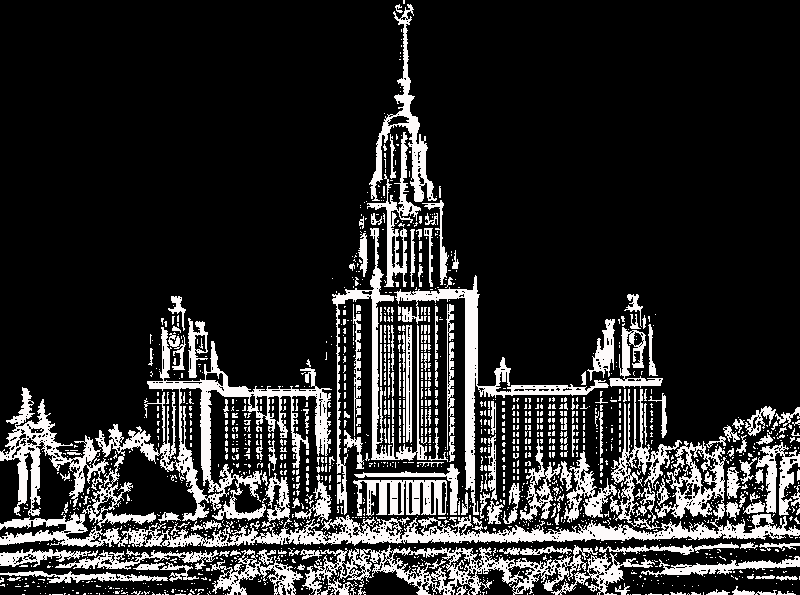
\includegraphics[width=1.2\linewidth]{images/msu_binary.png}} Бинарное \\
		\end{minipage}
		\hfill
		\begin{minipage}[h]{0.25\linewidth}
			\center{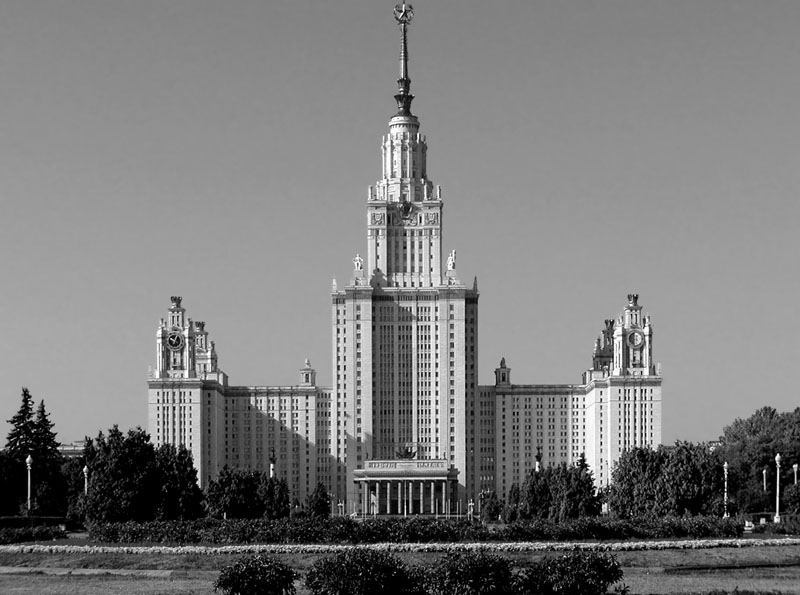
\includegraphics[width=1.2\linewidth]{images/msu_grayscale.png}} Серое\\
		\end{minipage}
		\hfill
		\centering
		\begin{minipage}[h]{0.25\linewidth}
			\center{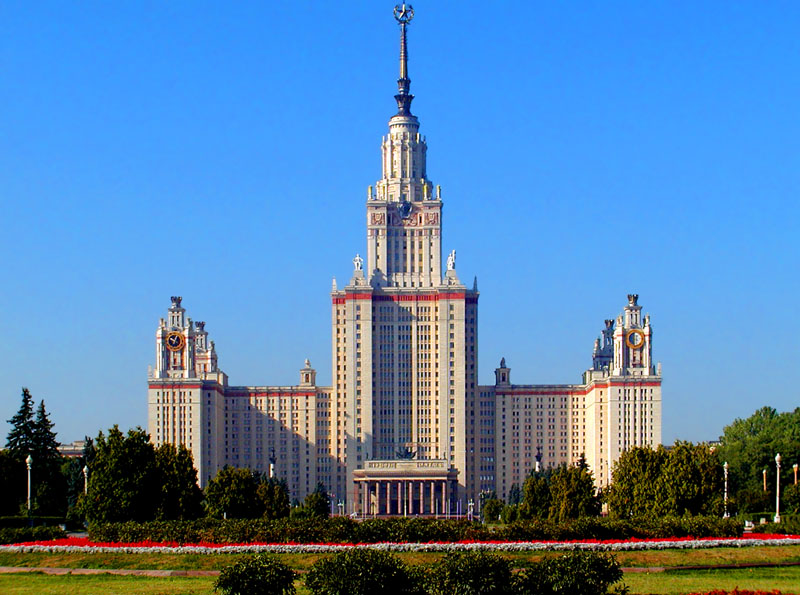
\includegraphics[width=1.2\linewidth]{images/msu.png}} Цветное \\
		\end{minipage}
		
		
		\label{fig:image}
	\end{figure}
	
	
\end{frame}

\begin{frame}[fragile]\frametitle{Пример: устранение шума}

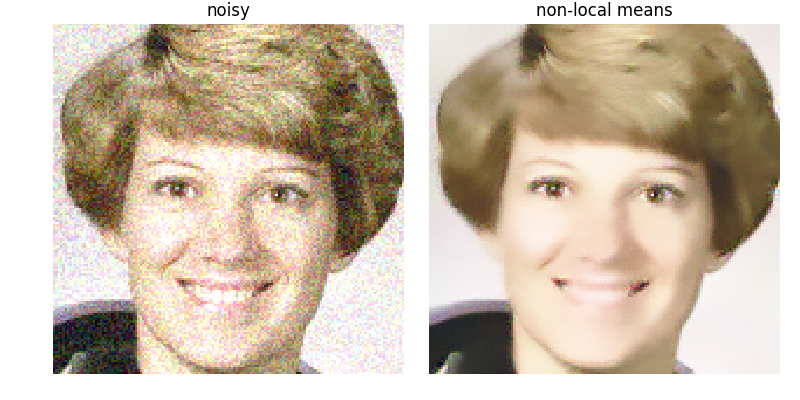
\includegraphics[scale=0.5]{images/noize_removal.png}

\href{http://scikit-image.org/docs/dev/auto_examples/filters/plot_nonlocal_means.html#sphx-glr-auto-examples-filters-plot-nonlocal-means-py}{http://scikit-image.org/docs/dev/auto\_examples/filters/...}
\end{frame}

\begin{frame}[fragile]\frametitle{Пример: выделение краёв}

\centering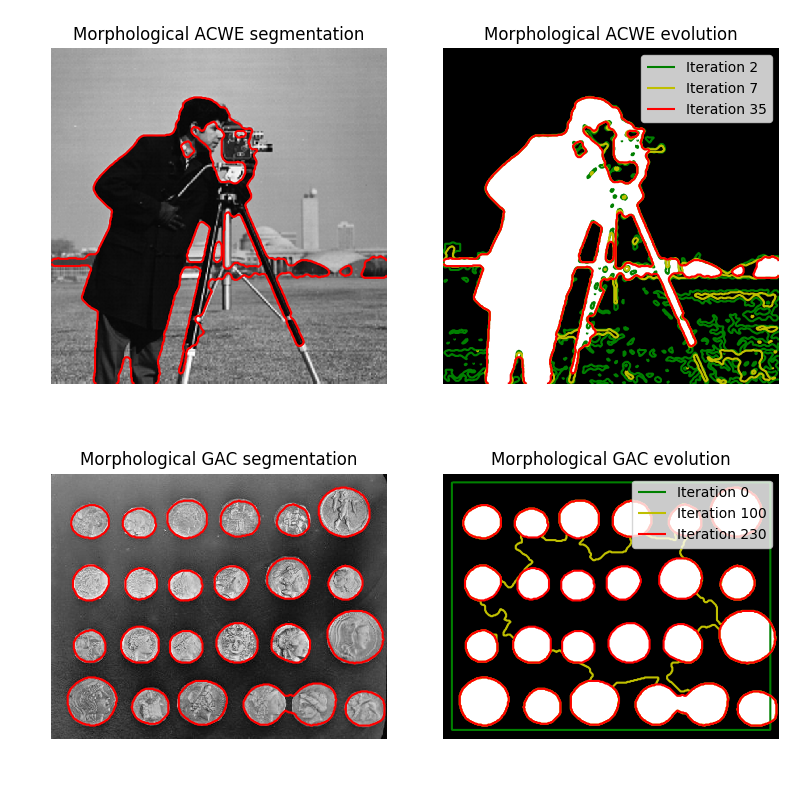
\includegraphics[scale=0.35]{images/segmentation.png}

\href{http://scikit-image.org/docs/dev/auto_examples/segmentation/plot_morphsnakes.html#sphx-glr-auto-examples-segmentation-plot-morphsnakes-py}{http://scikit-image.org/docs/dev/auto\_examples/segmentation/...}
\end{frame}

\begin{frame}[fragile]\frametitle{Пример: изменение баланса цвета}
\centering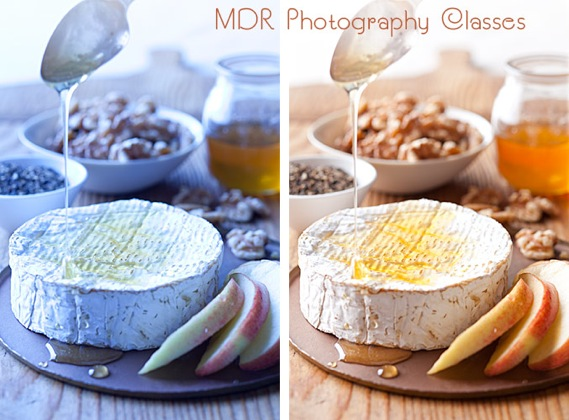
\includegraphics[scale=0.35]{images/balance.jpg}

\hfill

\href{http://studioeszkozok.hu/uploads/images/7631179_1497473781_color-temp.jpg}{http://studioeszkozok.hu/uploads/images/...}
\end{frame}

\begin{frame}[fragile]\frametitle{Зачем нужна обработка изображений?}
\begin{enumerate}
\item Улучшение изображения для восприятия человеком
(изображение должно стать «лучше» с субъективной точки зрения
человека)
\item \textbf{Улучшение изображения для восприятия компьютером}

\textbf{(улучшение качества работы алгоритмов)}

\item Технические нужды (например, уменьшение размера изображений для пересылки по почте)

\item Построение спецэффектов
\end{enumerate}

\hfill

Обо всём этом подробнее в курсах <<Обработка и распознавание изображений>> и <<Компьютерная графика>>

\end{frame}

\begin{frame}[fragile]\frametitle{Улучшение качества работы алгоритма на изображениях}

\begin{itemize}
\item Предобработка входных изображений

\begin{itemize}
\item Удаление шума, преобразование цветов
\end{itemize}

\item Постобработка изображений

\begin{itemize}
	\item Удаление шумовых объектов, отверстий
\end{itemize}

\item Выделение дополнительных признаков

\begin{itemize}
\item Выделение важных объектов, областей
\end{itemize}
%\item Генерация дополнительных изображений для обучения
%
%\begin{itemize}
%\item Добавление изображений, полученных из исходных с помощью некоторых преобразований 
%
%\end{itemize}

\item Аугментация объектов

\begin{itemize}
\item Преобразование объектов в ходе обучения/применения модели

\end{itemize}

\end{itemize}
\end{frame}

\begin{frame}[fragile]\frametitle{Пример: классификация цифр}
Первое практическое задание: классификация датасета MNIST

\hfill

\begin{center}
{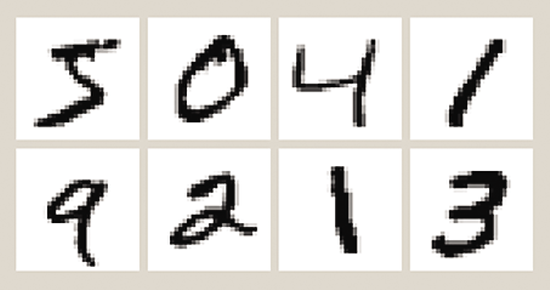
\includegraphics[scale=1]{images/mnist.png}}
\end{center}

\hfill

Класс изображения не меняется при:
\begin{itemize}
\item сдвигах на 1-10 пикселей

\item поворотах на 10-15 градусов в каждую из сторон

\item размытии, удалении шумов
\end{itemize}

\hfill

Добавив преобразованные объекты в исходную выборку, можно существенно повысить качество
\end{frame}

\begin{frame}[fragile]\frametitle{Аугментация}
Часто используемые методы аугментации
\begin{itemize}
\item отражение
\item сдвиг
\item поворот
\item масштабирование (увеличение)
\item добавление шума, размытие
\item изменение яркости, контрастности, цветовой гаммы
\item удаление части изображения
\end{itemize}	


\href{https://medium.com/nanonets/how-to-use-deep-learning-when-you-have-limited-data-part-2-data-augmentation-c26971dc8ced}{\color{blue}{Хорошая статья по аугментации изображений}}

\end{frame}

\begin{frame}[fragile]\frametitle{Пример: классификация типов крыш}
Задача: определение типа крыши, один из четырёх классов:

\hfill

\begin{minipage}{0.49\linewidth}
\begin{enumerate}
\item North-South orientation

\item East-West orientation

\item Flat roof

\item Other
\end{enumerate}
\end{minipage}
\begin{minipage}{0.49\linewidth}
{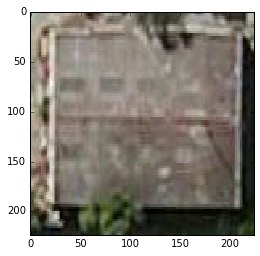
\includegraphics[scale=0.3]{images/roof.png}}
\end{minipage}

\hfill

\begin{enumerate}
\item При повороте на $90^\circ$ объект 1 и 2 класса меняет класс.

\item При повороте на $180^\circ$ объект 1 и 2 класса не меняет класс.

\item При повороте на $90^\circ$ объект 3 класса не меняет класс.
\end{enumerate}

\hfill

Аугментация объектов улучшила точность с $80\%$ до $84\%$
\end{frame}



\begin{frame}[fragile]\frametitle{Пример: детектирование действий водителя}
Детектировать запрещённые действия водителей по видео:

\hfill

\begin{minipage}{0.49\linewidth}
Исходное изображение:

{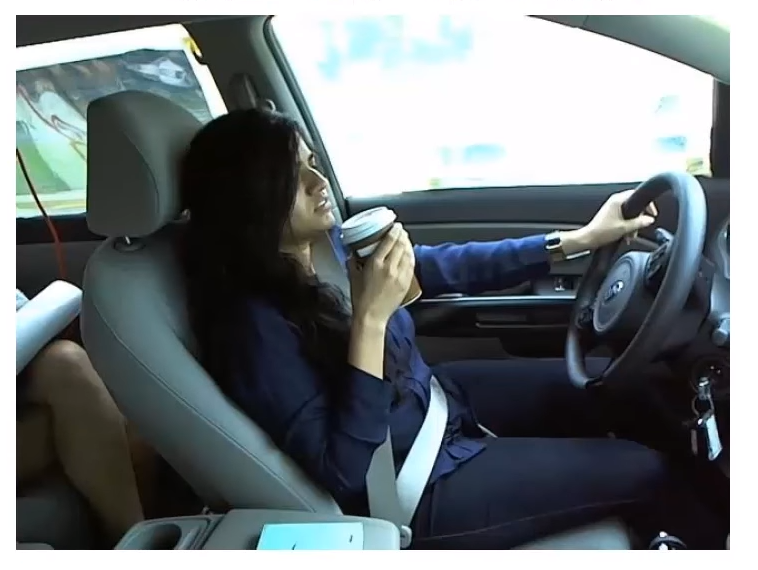
\includegraphics[scale=0.3]{images/girl_car.png}}
\end{minipage}
\begin{minipage}{0.49\linewidth}
Выделение~областей:

{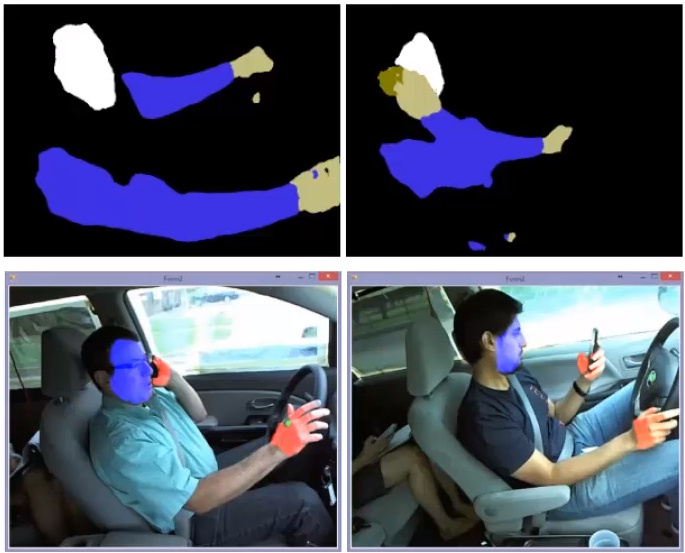
\includegraphics[scale=0.3]{images/faces_car.png}}
\end{minipage}

\hfill

Алгоритм можно настраивать отдельно на выделенные области

\end{frame}


\begin{frame}[fragile]\frametitle{Библиотека scipy}
\begin{itemize}
\item Scipy --- библиотека для научных вычислений

\href{https://scipy.org/}{https://scipy.org/}

\item В том числе, есть несколько модулей для работы с изображениями (misc, ndimage)

\item Только самые базовые алгоритмы
\end{itemize}
\end{frame}


\begin{frame}[fragile]\frametitle{Библиотека scikit-image}
\begin{itemize}
\item Scikit-image --- библиотека для работы с изображениями

\href{http://scikit-image.org/}{http://scikit-image.org/}

\item Большое количество реализованных алгоритмов для работы с изображениями
\item Много выложенных примеров использования библиотеки, но плохая документация
\end{itemize}
\end{frame}

\begin{frame}[fragile]\frametitle{Библиотека OpenCV}
\begin{itemize}
\item OpenCV --- продвинутая библиотека для компьютерного зрения, есть хороший интерфейс для Python 2.7

\href{https://opencv-python-tutroals.readthedocs.io/en/latest/index.html}{https://opencv-python-tutroals.readthedocs.io/en/latest/index.html}

\item Огромное количество реализованных алгоритмов для работы с изображениями, видео, 3D моделями 

\item Хорошая документация
\end{itemize}
\end{frame}

\section{Работа с изображениями в Python}
\subsection*{}

\begin{frame}[fragile]\frametitle{Представление изображения в памяти (scipy)}
\begin{pcode}
>>> import matplotlib.pyplot as plt
>>> %matplotlib inline
>>> import scipy.misc as misc
...
>>> img = misc.imread('msu.png') # загрузка изображения
>>> print(type(img))  # изображение — трёхмерный numpy array
<class numpy.ndarray>
>>> print(img.shape)
(595, 800, 3)
>>> plt.imshow(img)
\end{pcode}

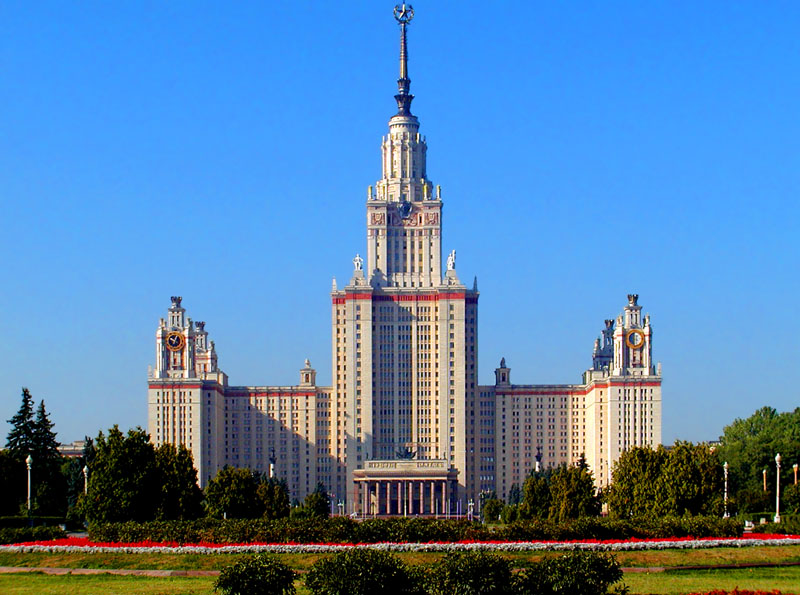
\includegraphics[scale=0.3]{images/msu.png}
\end{frame}

\begin{frame}[fragile]\frametitle{Представление изображения в памяти (skimage)}
То же самое, но с scikit-image:
\begin{pcode}
>>> import skimage.io as io
...
>>> img = io.imread('msu.png') # загрузка изображения
>>> print(type(img))  # изображение — трёхмерный numpy array
<class numpy.ndarray>
>>> print(img.shape)
(595, 800, 3)
>>> plt.imshow(img)
\end{pcode}

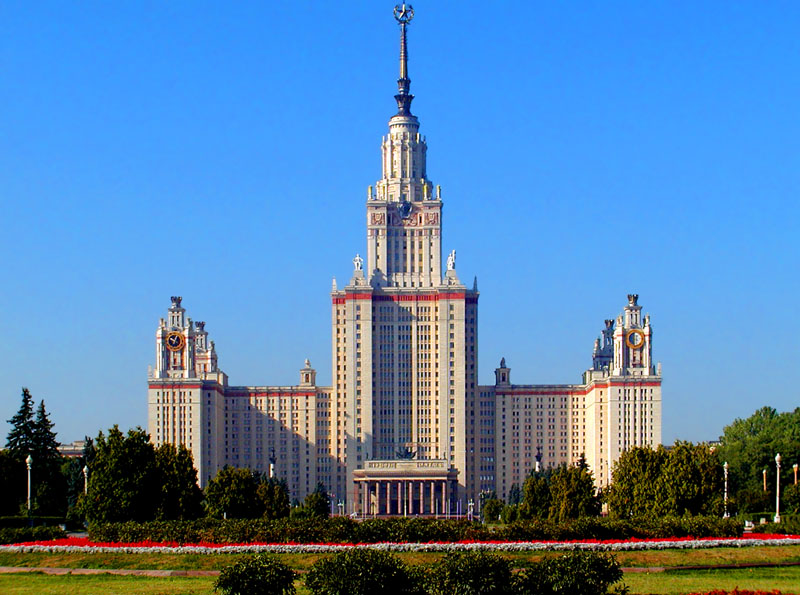
\includegraphics[scale=0.3]{images/msu.png}
\end{frame}

\begin{frame}[fragile]\frametitle{Сдвиги изображений}
\begin{pcode}
>>> import scipy.ndimage as ndimage
...
>>> new_img = ndimage.shift(img, [150, 150, 0])
>>> plt.imshow(new_img)
\end{pcode}
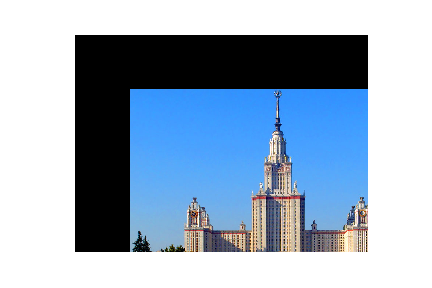
\includegraphics[scale=0.45]{images/img_shift.png}

\end{frame}

\begin{frame}[fragile]\frametitle{Повороты изображений (scipy)}
\begin{pcode}
>>> new_img = misc.imrotate(img, 90)
>>> plt.imshow(new_img)
\end{pcode}
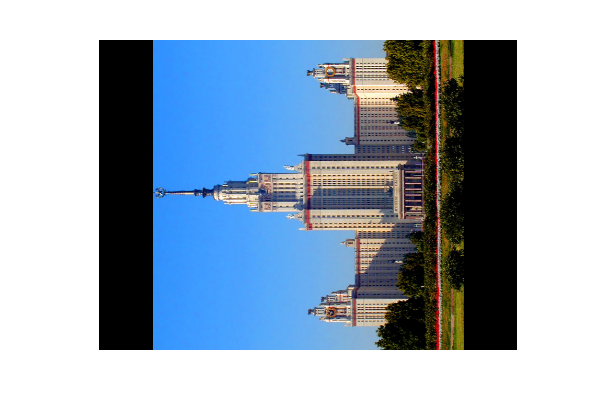
\includegraphics[scale=0.4]{images/img_rot_scipy.png}

Изображение обрезается, нельзя сохранить исходные пропорции, нельзя обрезать границы.

\end{frame}

\begin{frame}[fragile]\frametitle{Повороты изображений (skimage)}
\begin{pcode}
>>> import skimage.transform as transform
>>> new_img = transform.rotate(img, 90, resize=True)
>>> plt.imshow(new_img)
\end{pcode}
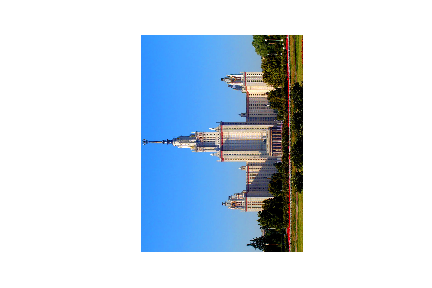
\includegraphics[scale=0.45]{images/img_rot_skimage.png}

Много параметров:
\begin{pcode}
transform.rotate(image, angle, resize=False, center=None, 
order=1, mode='constant', cval=0, clip=True,
reserve_range=False)
\end{pcode}

\end{frame}




\begin{frame}[fragile]\frametitle{Оттенки серого}
\begin{pcode}
>>> import skimage.color as color
>>> grey_img = color.rgb2grey(img)
>>> plt.imshow(grey_img, cmap=plt.cm.Greys)
\end{pcode}
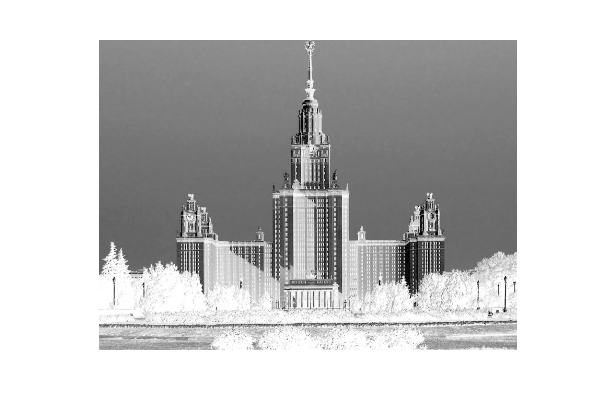
\includegraphics[scale=0.45]{images/img_grey.png}

\pause{
Формула для преобразования:
\[
Y =  0.299 R + 0.587 G + 0.114 B
\]
}
\end{frame}

\begin{frame}[fragile]\frametitle{Бинаризация изображений}
Бинаризация --- перевод изображения в черно-белое

\hfill

Бинаризация бывает:
\begin{itemize}
    \item Глобальная (один порог для всех пикселей)
    \item Локальная (порог зависит от положения пикселя)
    \item Адаптивная (порог зависит от положения и от яркости пикселя)
\end{itemize}
\end{frame}

\begin{frame}[fragile]\frametitle{Бинаризация в opencv}
\begin{pcode}
    >>> import cv2 as cv
    >>> th1, glob_bin_img = cv.threshold(
    ...     grey_img, 0.5, 1, cv.THRESH_BINARY
    ... )
    >>> adaptive_bin_img = cv.adaptiveThreshold(
    ...     img_tmp, 255, cv.ADAPTIVE_THRESH_MEAN_C,
    ...     cv.THRESH_BINARY, 5, 5
    ... )
\end{pcode}

\begin{minipage}{0.49\linewidth}
    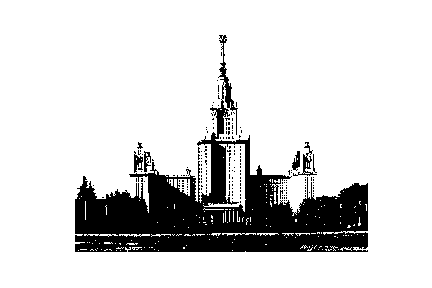
\includegraphics[scale=0.35]{images/img_global_binarization}
\end{minipage}
\begin{minipage}{0.49\linewidth}
    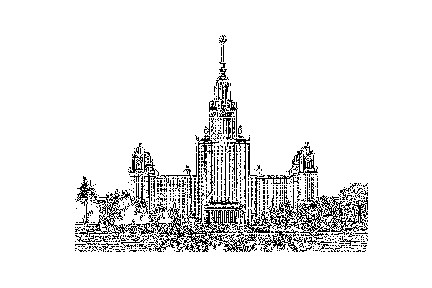
\includegraphics[scale=0.35]{images/img_adaptive_binarization}
\end{minipage}
\end{frame}




\begin{frame}[fragile]\frametitle{Медианный фильтр}
Медианный фильтр --- возвращает медианное значение по окну

\begin{center}
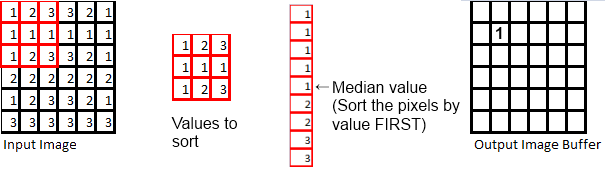
\includegraphics[scale=0.5]{images/sorting-median}
\end{center}

Является нелинейным фильтром (нельзя выразить с помощью линейных операций от входа).
\end{frame}


\begin{frame}[fragile]\frametitle{Удаление шумов с помощью медианного фильтра}
\begin{pcode}
>>> noise_coords_i = np.random.randint(0, img.shape[0], 50000)
>>> noise_coords_j = np.random.randint(0, img.shape[1], 50000)
>>> img_copy = np.copy(grey_img)
>>> img_copy[noise_coords_i, noise_coords_j] = 0
...
>>> blur_img = filters.median(img_copy)
\end{pcode}

\begin{minipage}{0.49\linewidth}
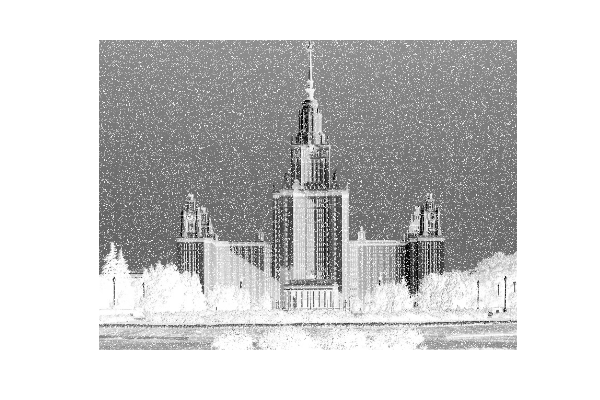
\includegraphics[scale=0.4]{images/img_noize.png}
\end{minipage}
\begin{minipage}{0.49\linewidth}
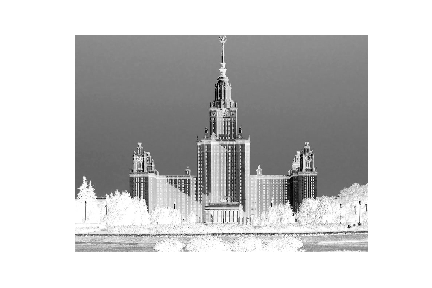
\includegraphics[scale=0.4]{images/img_median.png}
\end{minipage}
\end{frame}

\begin{frame}[fragile]\frametitle{Гауссовский фильтр (gaussian blur)}

Можно применять гауссовский фильтр, чтобы сгладить/размыть изображение (является линейным):

\[
Y[i, j] = \sum_{l = -k}^k \sum_{m = -k}^k X[i + l, j + m] \frac{1}{\sqrt{2 \pi \sigma}} \exp\left(-\frac{\sqrt{l^2 + m^2}}{2\sigma^2}\right)
\]

\hfill

\begin{pcode}
>>> blur_image = filters.gaussian_filter(img, sigma=5)
\end{pcode}

\begin{center}
    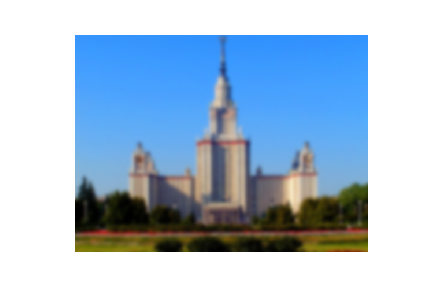
\includegraphics[scale=0.4]{images/blur}
\end{center}

\end{frame}

\begin{frame}[fragile]\frametitle{Пример: бейзлайн для выделения границ документа}
\centering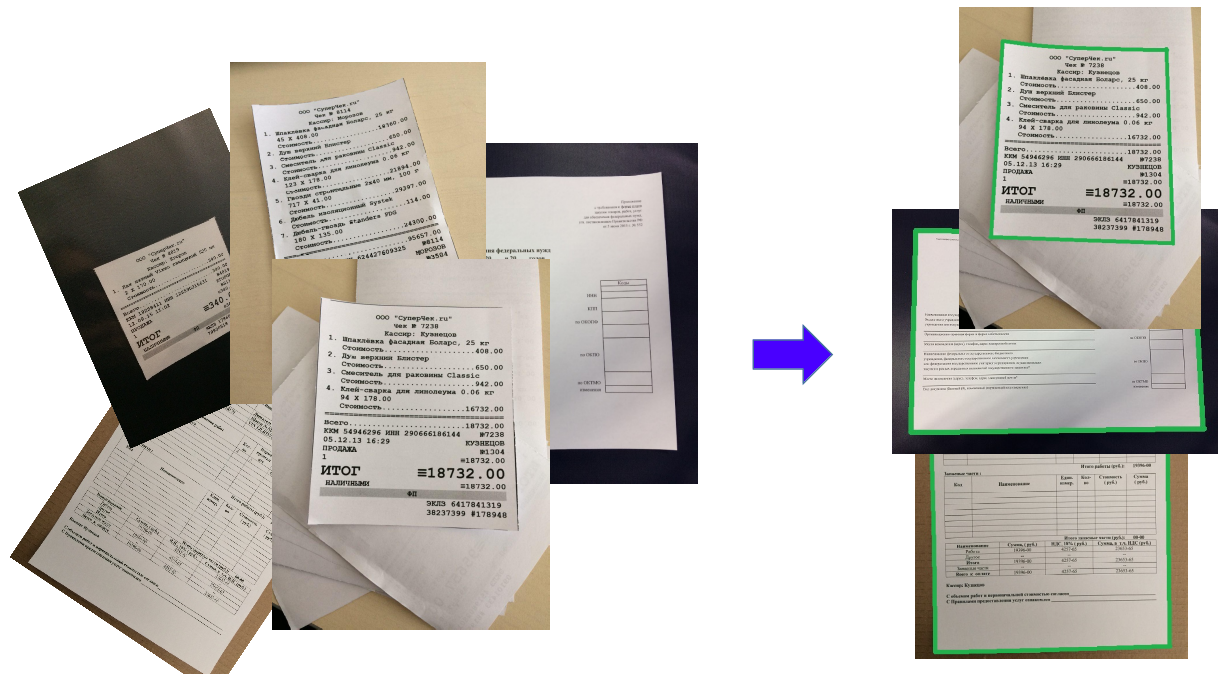
\includegraphics[scale=0.35]{images/docs_processing.png}
\end{frame}

\begin{frame}[fragile]\frametitle{Пример: бейзлайн для выделения границ документа}
\begin{enumerate}
    \item Сглаживание
    \item Бинаризация
    \item Удаление небольших черных областей
    \item Удаление небольших белых областей
    \item Аппроксимация четырехугольником
    \item Восстановления порядка вершин
    \item Вырезание документа
\end{enumerate}

\end{frame}

\begin{frame}[fragile]\frametitle{Пример: бейзлайн для выделения границ документа}
\begin{center}
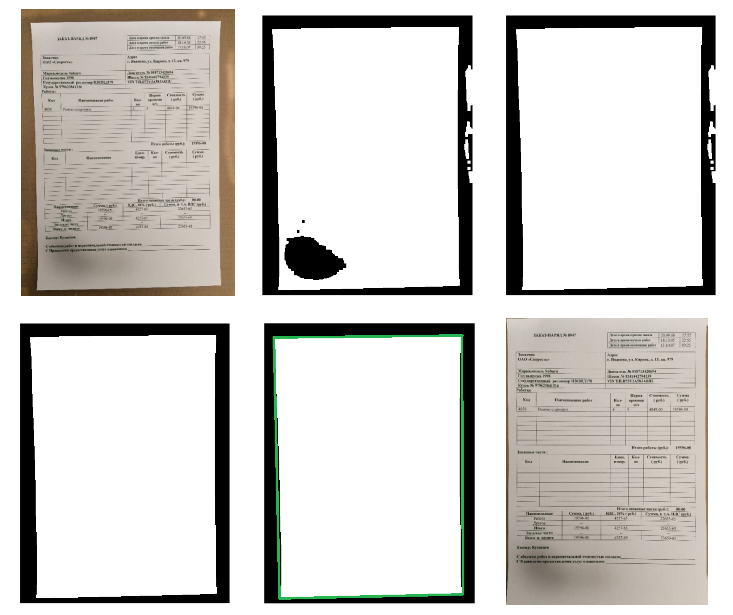
\includegraphics[scale=0.4]{images/img_doc.png}
\end{center}
\end{frame}

\begin{frame}[fragile]\frametitle{Заключение}
\begin{itemize}
\item Используя методы обработки изображений, можно повысить качество работы алгоритма

\item Используя классические подходы, можно получить бейзлайн решения даже для сложных задач

\item В Python есть несколько библиотек с уже реализованными алгоритмами обработки

\item У многих библиотек есть свои встроенные средства обработки 
\end{itemize}
\end{frame}


\end{document}